%!TEX root = ../my_thesis.tex
\chapter{Techniques for fast z feedback}

\section{Double PID}

\section{Tilt compensation}

If the probe/sample angle is not perpendicular, we observe a tilt on the surface. This tilt is problematic when it becomes larger than the features. Flattening algorithms restore the image and put the data on the same level. This technique works if the range of the tip is large enough. We have decided to take another approach and to dynamically compensate for the tilt.

First, we scan the surface of the sample with a circle pattern. It gives us informations about the general topography of the surface. Then, we compute the plane equation of the surface by applying a fit in Igor Pro.

\begin{equation}\label{eqn:planeeq}
z = a_1 x + a_2 y + a_3 
\end{equation}

Igor Pro finds the coefficients by minimizing the values of Chi-Square. We generate the waves to send to the controller the following way.

\begin{equation}\label{eqn:sendwave}
wavetosend = a_1 wavex + a_2 wavey 
\end{equation}

\subsection{Experiment}

We took a calibration sample to test the efficiency of our method.


\begin{figure}[H]
  \centering
  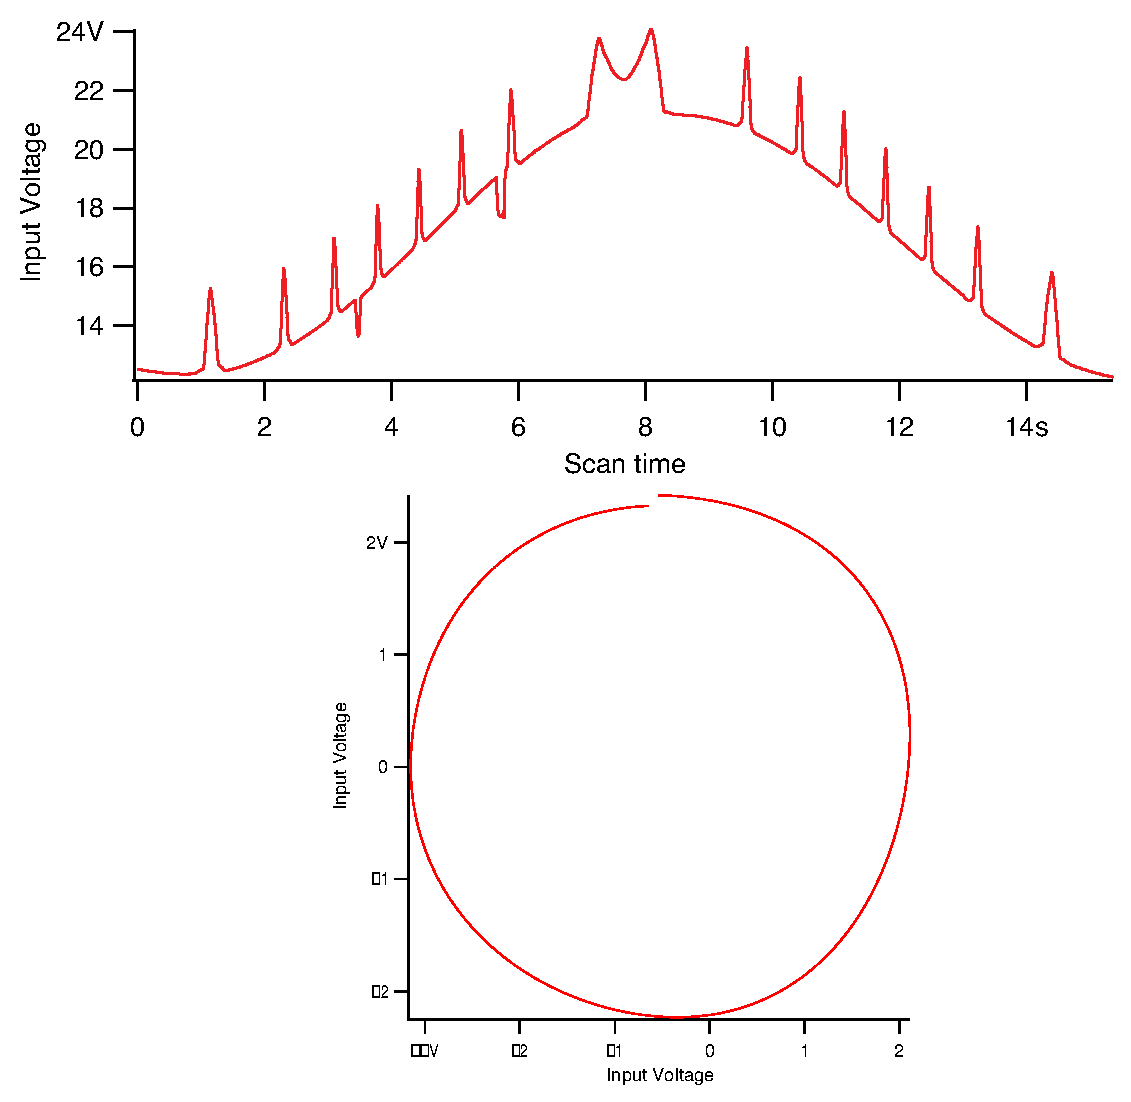
\includegraphics[scale=0.1]{images/tiltcircles.eps}
    \caption{Output of the tilt pattern}
  \label{tiltcircle}
\end{figure}

When we scanned the surface on our plane we had the following coefficients for the plane.


\begin{table}[H]
\caption{Planefit coefficients} % title of Table
\centering % used for centering table
\begin{tabular}{c c c} % centered columns (4 columns)
\hline\hline %inserts double horizontal lines
$a_1$ & $a_2$ & $a_3$ \\ [0.5ex] % inserts table 
%heading
\hline % inserts single horizontal line
-0.14615  & -0.031882 & 29.537 \\[1ex]

\hline %inserts single line
\end{tabular}
\label{table:planefit} % is used to refer this table in the text
\end{table}

The size of the scan is 30 um and the spiral has 80 loops. The scan pattern we are going to send to the controller is generated with the previously computed planefit coefficients. 

\begin{figure}[H]
  \centering
  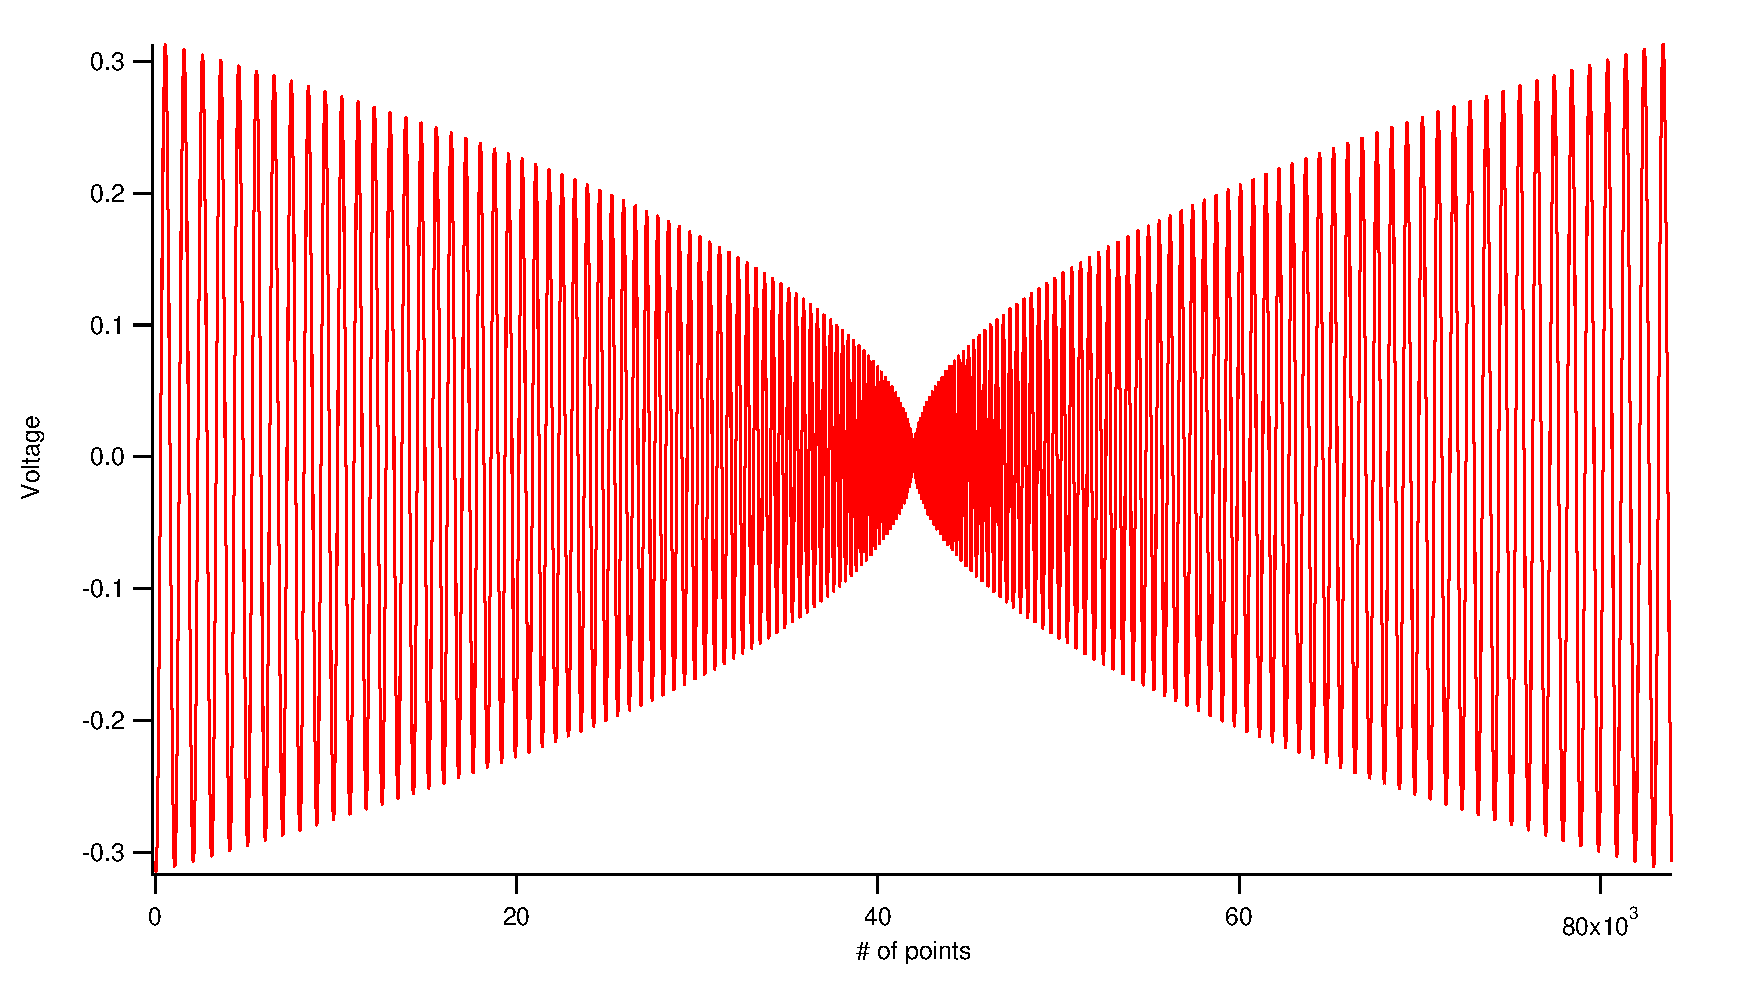
\includegraphics[scale=0.1]{images/spiralztiltout.eps}
    \caption{Input of the tilt compensation}
  \label{spiralztiltout}
\end{figure}



\begin{figure}[H]
  \centering
  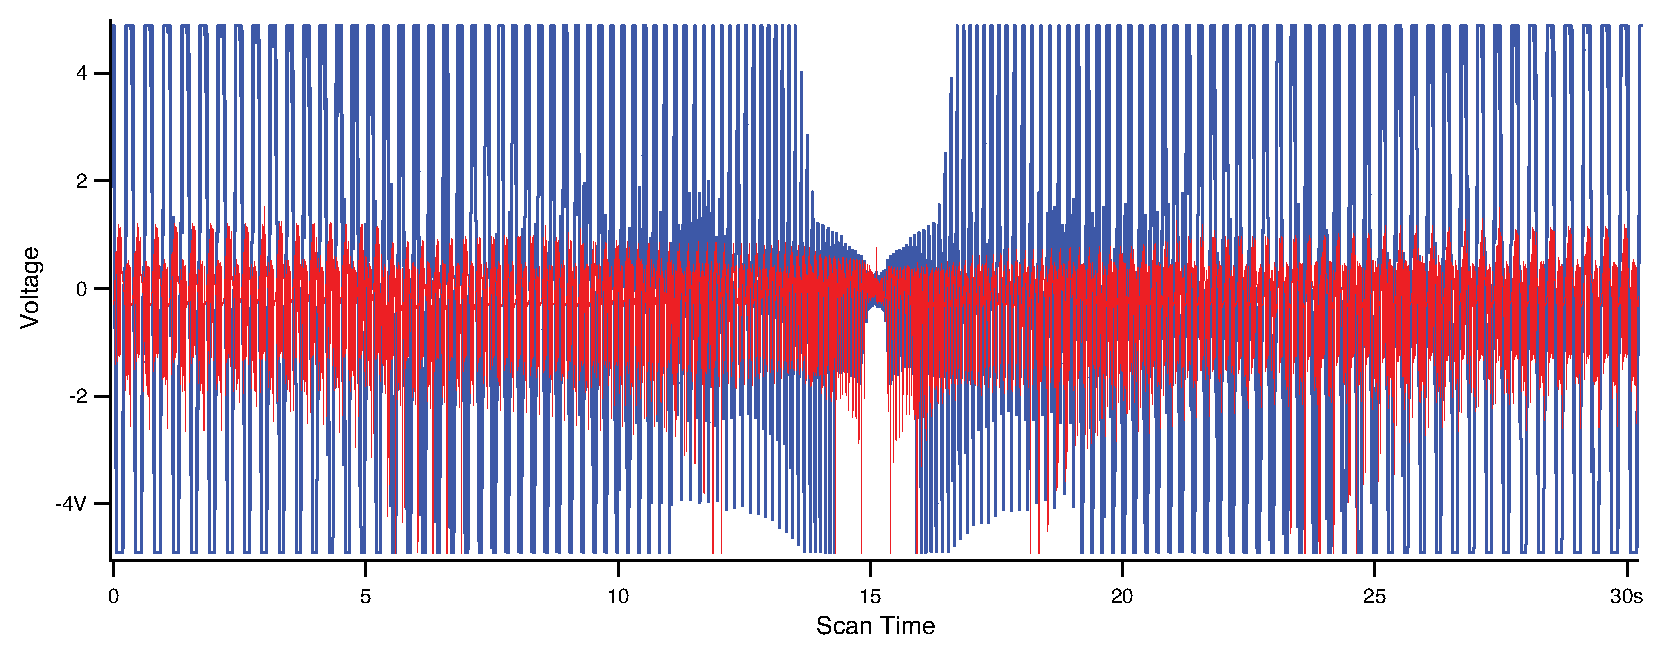
\includegraphics[scale=0.1]{images/tiltcorrectiongraph.eps}
    \caption{Output of the fast piezo}
  \label{spiralzfast}
\end{figure}


The tilt compensation will take a load off the small fast piezoelectrical ceramics. The Figure ~\ref{spiralzfast} shows the efficiency of our method. Indeed, the fast piezo was previously saturating. The piezos was trying to reach features that are larger than his range. If we use the tilt correction, we see that our piezo has no problem reaching those features.
